% Provenance (never printed): cycle 4 SVT/physique, "La planete Terre,
% l'environnement": uneven heating of the Earth, movements of the
% atmosphere, the global circulation and the climate zones; see
% sources/book1/PROVENANCE.md. Book 1, grade 8, chapter 2.
% Vocabulary guard: owns convection cell (atmospheric, descriptive), sea
% breeze and land breeze, the global winds, the global circulation. The
% Coriolis effect is told as "the Earth's rotation deflects"; Hadley and
% Ferrel cells and the intertropical convergence zone are named in prose
% only (Book 3 owns them); mantle convection is Book 2's.
\chapter{Winds and the Global Circulation}\label{ch:g8:winds-global-circulation}

For centuries, sailing ships leaving the ports of Europe and Africa for
the Americas relied on a steady wind from the east, which blows on both
sides of the \omterm{def:g3:continents-and-oceans:equator}{equator} and carried them across the Atlantic. Sailors all
over the world knew it, and the early trade with the Americas depended on
it: it is the \emph{trade wind}. Even now, cargo ships use the \omterm{def:g8:winds-global-circulation:global-winds}{trade
winds}, and the \omterm{def:g2:water-on-earth:ocean}{ocean} currents they drive, to shorten their voyages.
% ledger: nos:trade-winds

\begin{omfigure}
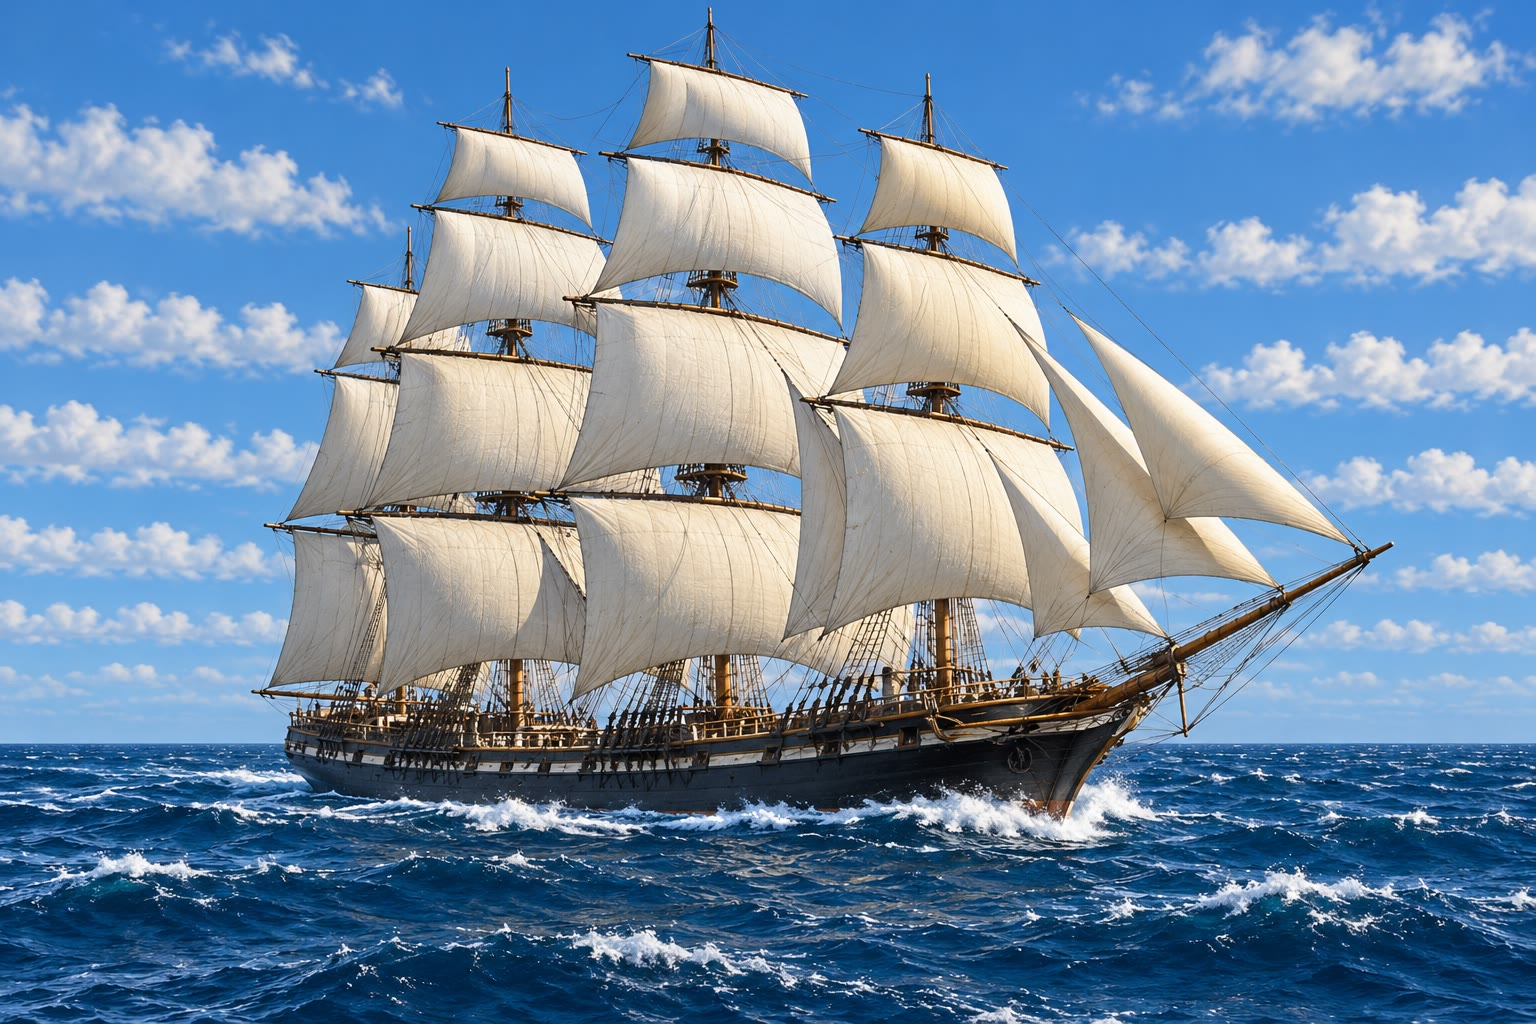
\includegraphics[width=0.62\linewidth]{images/book1/ai/g8-sailing-ship.jpg}

{\small A sailing ship running before a steady wind on the open \omterm{def:g2:water-on-earth:ocean}{ocean}
(AI-generated illustration of a generic scene).}
\label{fig:g8:winds-global-circulation:ship}
\end{omfigure}

Why does the trade wind blow from the east, and always in the same
places? Why are there \omterm{def:g5:weather-and-climate:desert}{deserts} near the \omterm{def:g5:weather-and-climate:tropics}{tropics} and \omterm{def:g5:weather-and-climate:rainforest}{rainforests} near the
\omterm{def:g3:continents-and-oceans:equator}{equator}? The answer starts with the Sun.

\begin{recall}
Wind is air in motion (the physics books). Air presses on everything it
touches, and the pressure falls with height
(\cref{ch:g8:the-atmosphere}). The \omterm{def:g1:watching-the-weather:weather}{weather} happens in the \omterm{def:g8:the-atmosphere:layers}{troposphere},
the lowest layer of the atmosphere. The Earth has \omterm{def:g5:weather-and-climate:climate-zone}{climate zones}: hot and
wet near the \omterm{def:g3:continents-and-oceans:equator}{equator}, with \omterm{def:g5:weather-and-climate:rainforest}{rainforests}; hot and dry \omterm{def:g5:weather-and-climate:desert}{deserts} near the
\omterm{def:g5:weather-and-climate:tropics}{tropics}; temperate, then cold zones towards the \omterm{def:g3:continents-and-oceans:poles}{poles}
(\cref{ch:g5:weather-and-climate}).
\end{recall}

\section{The Sun heats the Earth unevenly}

At noon on the day of an equinox, the Sun is straight overhead at the
\omterm{def:g3:continents-and-oceans:equator}{equator}. Its rays arrive steeply there and fall on a small patch of
ground. Further north or south, the same rays arrive at a slant and are
spread over a larger patch: each square metre receives less of their
energy. At \omterm{def:g6:latitude-longitude:latitude}{latitude} \ang{60}, the same beam covers twice the ground it
covers at the \omterm{def:g3:continents-and-oceans:equator}{equator}, so each square metre gets half as much.
% ledger: (geometry: figdata/grade-8/sunlight_spread.py, spread = 1/cos(latitude))

\begin{omfigure}
\begin{tikzpicture}[font=\footnotesize]
  \def\R{2.6}\def\w{0.2}
  \fill[blue!10] (0,0) circle (\R);
  \draw (0,0) circle (\R);
  \draw[black!50] (-\R,0) -- (\R,0);
  \draw[black!40, dashed] (0,0) -- (60:\R);
  \draw[black!40] (0,0) ++(0:0.7) arc (0:60:0.7);
  \node at (25:0.95) {\ang{60}};
  \node[anchor=east, black!60] at (-\R-0.05,0) {equator};
  % beam at the equator: rays between y = -w and y = w
  \foreach \y in {-0.2,-0.1,0,0.1,0.2} {
    \pgfmathsetmacro{\x}{sqrt(\R*\R-\y*\y)}
    \draw[orange!80!black, -{Stealth[length=1.6mm]}] (6.2,\y) -- (\x+0.03,\y);}
  \draw[omThm, line width=2.2pt] ({sqrt(\R*\R-0.35*0.35)},-0.35) arc ({asin(-\w/\R)}:{asin(\w/\R)}:\R);
  % beam near 60 degrees: rays between y = R sin 60 - w and + w
  \pgfmathsetmacro{\yc}{\R*sin(60)}
  \foreach \d in {-0.2,-0.1,0,0.1,0.2} {
    \pgfmathsetmacro{\y}{\yc+\d}
    \pgfmathsetmacro{\x}{sqrt(\R*\R-\y*\y)}
    \draw[orange!80!black, -{Stealth[length=1.6mm]}] (6.2,\y) -- (\x+0.03,\y);}
  \draw[omThm, line width=2.2pt] ({sqrt(\R*\R-(\yc-\w)^2)},\yc-\w) arc ({asin((\yc-\w)/\R)}:{asin((\yc+\w)/\R)}:\R);
  \node[anchor=west, align=left] at (6.3,0) {the same beam\\on a small patch};
  \node[anchor=west, align=left] at (6.3,\yc) {the same beam spread\\over twice the ground};
\end{tikzpicture}

{\small Two identical beams of sunlight at noon on an equinox. At the
\omterm{def:g3:continents-and-oceans:equator}{equator} they fall straight down on a small patch (thick line); at
\ang{60} of \omterm{def:g6:latitude-longitude:latitude}{latitude} they slant and cover twice as much ground.}
% ledger: (geometry: figdata/grade-8/sunlight_spread.py)
\label{fig:g8:winds-global-circulation:beams}
\end{omfigure}

\begin{center}\small
\begin{tabular}{|l|c|c|c|c|c|}
\hline
\omterm{def:g6:latitude-longitude:latitude}{latitude} & \ang{0} & \ang{30} & \ang{45} & \ang{60} & \ang{75} \\
\hline
ground covered by the same beam & 1 & 1.15 & 1.41 & 2 & 3.86 \\
\hline
energy per square metre (\% of the \omterm{def:g3:continents-and-oceans:equator}{equator}'s) & 100 & 87 & 71 & 50 & 26 \\
\hline
\end{tabular}
\end{center}
% ledger: (figdata/grade-8/sunlight_spread.py main table)

As the Earth goes round the Sun, its tilted axis makes the overhead Sun
move between the two \omterm{def:g5:weather-and-climate:tropics}{tropics}, which gives the seasons (the physics
books); but all year round, the regions near the \omterm{def:g3:continents-and-oceans:equator}{equator} receive much
more energy than those near the \omterm{def:g3:continents-and-oceans:poles}{poles}. This uneven heating is the main
driver of the winds: the atmosphere carries warm air towards the \omterm{def:g3:continents-and-oceans:poles}{poles}
and cold air towards the \omterm{def:g3:continents-and-oceans:equator}{equator}.
% ledger: mo:global-circ

\section{Rising and sinking air}

Warm air is lighter than cold air: it rises, and the cooler air around
flows in to take its place. Where air rises, it presses less on the
ground: the pressure there is low. Where air sinks, it presses more: the
pressure is high. At the ground, the wind blows from high pressure
towards low pressure. Rising, cooling, sinking and flowing back, the air
turns in a loop.
% ledger: jetstream:sea-breeze, mo:three-cells

\begin{definition}[Convection cell]\label{def:g8:winds-global-circulation:convection-cell}
A \emph{convection cell}\index{convection cell} in the atmosphere is a
loop of moving air: air warmed from below rises, spreads out at height,
cools and sinks somewhere else, and flows back along the ground to where
it rose. Under the rising air the pressure is low; under the sinking air
it is high.
\end{definition}
% ledger: jetstream:sea-breeze, mo:three-cells

\begin{inthelab}[Warm air rises]
Indoors, cut a spiral out of a sheet of thin paper, like the peel of an
apple, and hang it by its centre on a thread. Hold it high above a warm
radiator in winter (never above a flame or a candle): it slowly starts to
turn. The air warmed by the radiator rises and pushes on the spiral. Hold
it near a cold window: does it turn the other way, or not at all?
\end{inthelab}

The smallest \omterm{def:g8:winds-global-circulation:convection-cell}{convection cells} can be felt on a sunny day at the seaside.
The land and the \omterm{def:g2:water-on-earth:ocean}{sea} receive the same sunshine, but the Sun's rays do
not go deep into the ground, while the \omterm{def:g2:water-on-earth:ocean}{sea} spreads its heat through a
thick layer of water. So the land warms up much more by day, and cools
down much more at night.
% ledger: jetstream:sea-breeze

\begin{omfigure}
\begin{tikzpicture}[font=\footnotesize, >={Stealth[length=2mm]}]
  \foreach \px/\title/\dir in {0/{By day: the sea breeze}/1, 8.3/{At night: the land breeze}/-1} {
    \begin{scope}[xshift=\px cm]
      \fill[omSea] (0,0) rectangle (3.5,0.45);
      \fill[omLithAlluv] (3.5,0) -- (3.5,0.45) -- (7,0.75) -- (7,0) -- cycle;
      \draw (0,0.45) -- (3.5,0.45) -- (7,0.75);
      \node[anchor=south] at (3.5,3.25) {\textbf{\title}};
      \node at (1.75,0.22) {sea};
      \node at (5.6,0.3) {land};
    \end{scope}}
  % day loop: surface sea -> land, rise over land, return aloft, sink over sea
  \draw[->, omDef, line width=1.1pt] (1.2,0.8) -- (5.2,0.95);
  \draw[->, omThm, line width=1.1pt] (5.8,1.1) -- (5.8,2.4);
  \draw[->, black!60, line width=1.1pt] (5.2,2.75) -- (1.2,2.75);
  \draw[->, omDef, line width=1.1pt] (0.6,2.4) -- (0.6,1.1);
  \node[omDef] at (3.2,1.25) {sea breeze};
  \node at (0.6,0.75) {\textbf{H}};
  \node at (5.8,0.95) {\textbf{L}};
  \fill[yellow!80!orange] (6.6,2.7) circle (0.25);
  \node[anchor=north, align=center] at (1.75,-0.1) {cooler sea};
  \node[anchor=north, align=center] at (5.3,-0.1) {warmer land};
  % night loop: surface land -> sea, rise over sea, return aloft, sink over land
  \begin{scope}[xshift=8.3cm]
    \draw[->, omDef, line width=1.1pt] (5.2,1.0) -- (1.2,0.8);
    \draw[->, omThm, line width=1.1pt] (0.6,1.1) -- (0.6,2.4);
    \draw[->, black!60, line width=1.1pt] (1.2,2.75) -- (5.2,2.75);
    \draw[->, omDef, line width=1.1pt] (5.8,2.4) -- (5.8,1.15);
    \node[omDef] at (3.2,1.3) {land breeze};
    \node at (0.6,0.75) {\textbf{L}};
    \node at (5.8,1.0) {\textbf{H}};
    \fill[black!25] (6.6,2.7) circle (0.25); \fill[white] (6.72,2.78) circle (0.21);
    \node[anchor=north, align=center] at (1.75,-0.1) {warmer sea};
    \node[anchor=north, align=center] at (5.3,-0.1) {colder land};
  \end{scope}
\end{tikzpicture}

{\small The \omterm{def:g8:winds-global-circulation:breezes}{sea breeze} and the \omterm{def:g8:winds-global-circulation:breezes}{land breeze}: two small \omterm{def:g8:winds-global-circulation:convection-cell}{convection cells}
that turn opposite ways. Red arrows: rising warm air; H and L: high and
low pressure at the ground. By day the loop reaches 1000 to
\qty{1500}{m} up.}
% ledger: jetstream:sea-breeze
\label{fig:g8:winds-global-circulation:breezes}
\end{omfigure}

\begin{definition}[Sea breeze and land breeze]\label{def:g8:winds-global-circulation:breezes}
A \emph{sea breeze}\index{sea breeze} is a wind that blows from the \omterm{def:g2:water-on-earth:ocean}{sea}
towards the land by day, when the land is warmer than the \omterm{def:g2:water-on-earth:ocean}{sea}. A
\emph{land breeze}\index{land breeze} blows from the land towards the \omterm{def:g2:water-on-earth:ocean}{sea}
at night, when the land has become colder than the \omterm{def:g2:water-on-earth:ocean}{sea}.
\end{definition}
% ledger: jetstream:sea-breeze

\begin{omfigure}
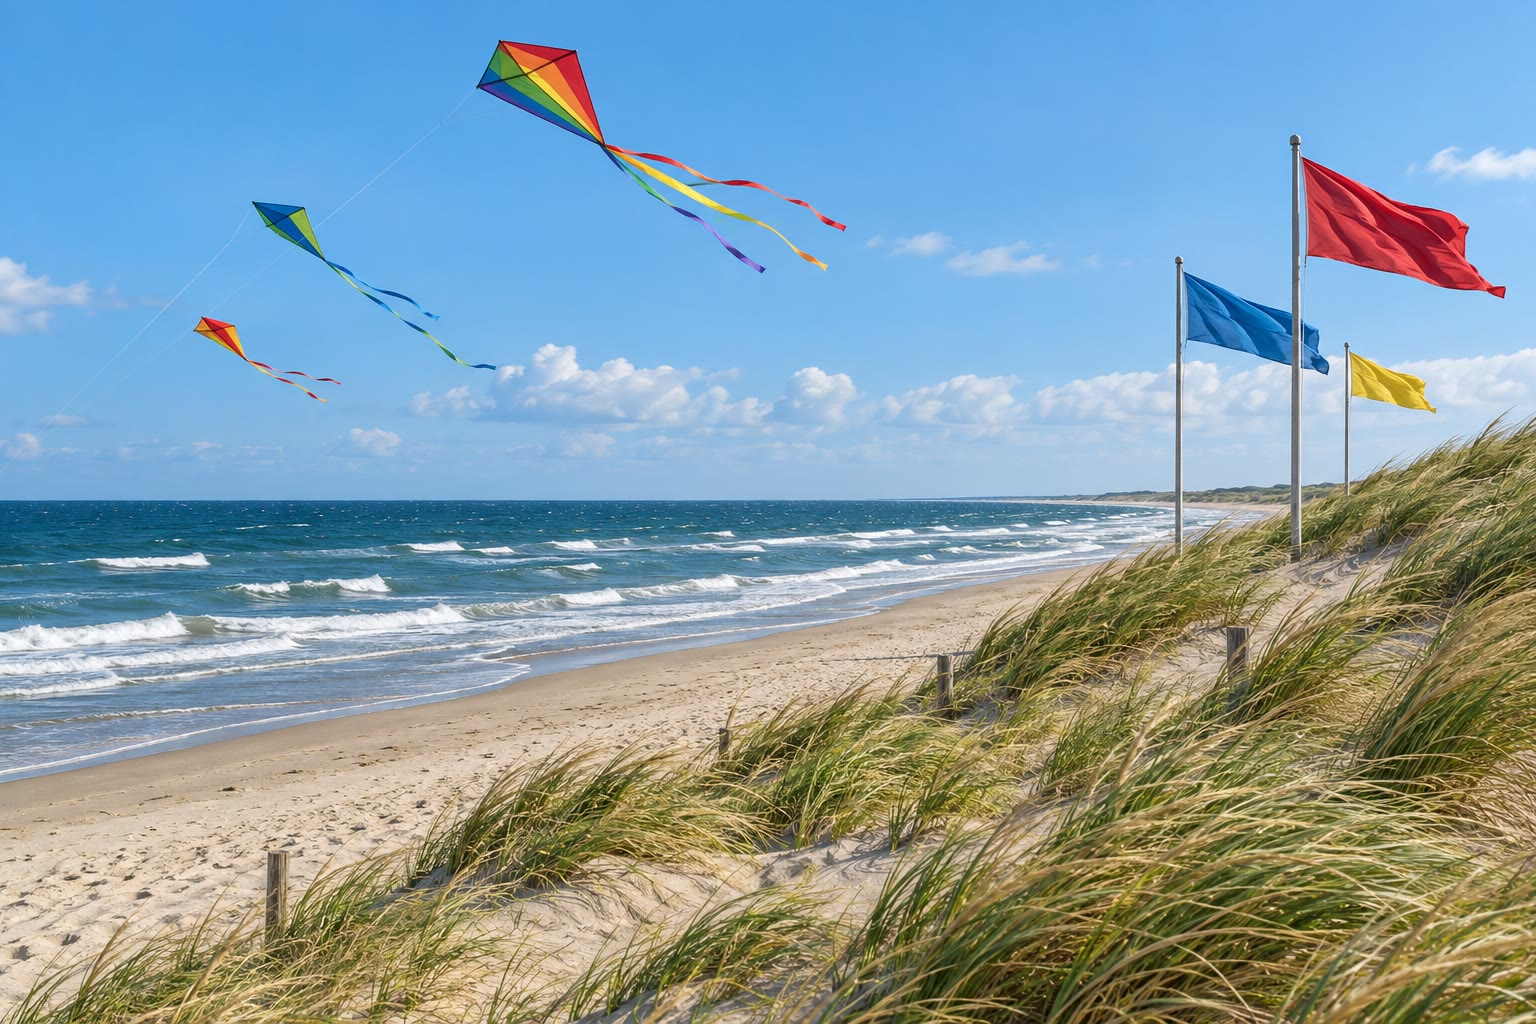
\includegraphics[width=0.55\linewidth]{images/book1/ai/g8-beach-kites.jpg}

{\small Kites flying in the afternoon wind on a beach (AI-generated
illustration of a generic scene).}
\label{fig:g8:winds-global-circulation:kites}
\end{omfigure}

\section{The global winds}

The same thing happens on the scale of the whole Earth. Near the
\omterm{def:g3:continents-and-oceans:equator}{equator}, the strongly heated air rises; it spreads towards the \omterm{def:g3:continents-and-oceans:poles}{poles} at
height and sinks again near \ang{30} of \omterm{def:g6:latitude-longitude:latitude}{latitude}. Averaged over many
years, the \omterm{def:g8:the-atmosphere:layers}{troposphere} of each \omterm{def:g3:continents-and-oceans:equator}{hemisphere} turns in three great \omterm{def:g8:winds-global-circulation:convection-cell}{convection
cells}: one from the \omterm{def:g3:continents-and-oceans:equator}{equator} to about \ang{30}, one from about \ang{30} to
about \ang{60}, and one from about \ang{60} to the \omterm{def:g3:continents-and-oceans:poles}{pole}. Meteorologists
call them the Hadley, Ferrel and polar cells. Their limits move with the
seasons, and the middle cell is a rough average of many passing \omterm{def:g5:natural-hazards:storm}{storms}.
% ledger: mo:three-cells, mo:global-circ, nos:doldrums

The winds that blow at the ground would go straight from high to low
pressure if the Earth did not turn. Because the Earth rotates, moving air
is turned aside: to the right in the \omterm{def:g3:continents-and-oceans:equator}{northern hemisphere}, to the left in
the \omterm{def:g3:continents-and-oceans:equator}{southern hemisphere}. So the air flowing back to the \omterm{def:g3:continents-and-oceans:equator}{equator} does not
come from the north, but from the north-east in the \omterm{def:g3:continents-and-oceans:equator}{northern hemisphere}
and from the south-east in the \omterm{def:g3:continents-and-oceans:equator}{southern hemisphere}.
% ledger: mo:global-circ, nos:trade-winds

\begin{definition}[The global winds]\label{def:g8:winds-global-circulation:global-winds}
The surface winds that blow most often in each belt of \omterm{def:g6:latitude-longitude:latitude}{latitude} are:
\begin{itemize}
  \item the \emph{trade winds}\index{trade winds}, between the \omterm{def:g3:continents-and-oceans:equator}{equator} and
        about \ang{30}, blowing from the north-east in the \omterm{def:g3:continents-and-oceans:equator}{northern
        hemisphere} and from the south-east in the \omterm{def:g3:continents-and-oceans:equator}{southern hemisphere};
  \item the \emph{westerlies}\index{westerlies}, between about \ang{30}
        and \ang{60}, blowing from the west (from the south-west in the
        \omterm{def:g3:continents-and-oceans:equator}{northern hemisphere}, from the north-west in the southern);
  \item the \emph{polar easterlies}\index{polar easterlies}, between about
        \ang{60} and the \omterm{def:g3:continents-and-oceans:poles}{poles}, blowing from the east.
\end{itemize}
\end{definition}
% ledger: nos:trade-winds, mo:three-cells, mo:global-circ

\begin{omfigure}
\begin{tikzpicture}[font=\scriptsize, >={Stealth[length=1.8mm]}]
  \def\R{3}
  \fill[blue!8] (0,0) circle (\R);
  \draw (0,0) circle (\R);
  \draw[black!45] (-\R,0) -- (\R,0);
  \foreach \l in {-60,-30,30,60} {
    \pgfmathsetmacro{\y}{\R*sin(\l)}
    \pgfmathsetmacro{\x}{\R*cos(\l)}
    \draw[black!45, dashed] (-\x,\y) -- (\x,\y);}
  % surface winds: NE trades, SW westerlies, NE polar easterlies (north); mirrored south
  \foreach \x in {-1.8,-0.6,0.6,1.8} {
    \draw[->, omThm, line width=0.9pt] (\x+0.35,0.95) -- (\x-0.35,0.55);
    \draw[->, omThm, line width=0.9pt] (\x+0.35,-0.95) -- (\x-0.35,-0.55);}
  \foreach \x in {-1.2,0,1.2} {
    \draw[->, omDef, line width=0.9pt] (\x-0.35,1.7) -- (\x+0.35,2.02);
    \draw[->, omDef, line width=0.9pt] (\x-0.35,-1.7) -- (\x+0.35,-2.02);}
  \foreach \x in {-0.4,0.4} {
    \draw[->, omMeth, line width=0.9pt] (\x+0.25,2.85) -- (\x-0.25,2.65);
    \draw[->, omMeth, line width=0.9pt] (\x+0.25,-2.85) -- (\x-0.25,-2.65);}
  \node[fill=blue!8, inner sep=1pt] at (0,1.2) {north-east trade winds};
  \node[fill=blue!8, inner sep=1pt] at (0,-1.2) {south-east trade winds};
  \node[fill=blue!8, inner sep=1pt] at (0,2.3) {westerlies};
  \node[fill=blue!8, inner sep=1pt] at (0,-2.3) {westerlies};
  \node[anchor=south] at (0,\R+0.05) {polar easterlies};
  \node[anchor=north] at (0,-\R-0.05) {polar easterlies};
  % pressure belts on the left
  \foreach \l/\t in {90/{H: sinking air}, 60/{L: rising air}, 30/{H: sinking air, dry, deserts}, 0/{L: rising air, clouds, rain}, -30/{H: sinking air, dry, deserts}, -60/{L: rising air}, -90/{H: sinking air}} {
    \pgfmathsetmacro{\y}{\R*sin(\l)}
    \pgfmathsetmacro{\x}{\R*cos(\l)}
    \draw[black!40] (-\x-0.05,\y) -- (-3.35,\y);
    \node[anchor=east] at (-3.4,\y) {\t};}
  \foreach \l/\t in {60/{\ang{60} N}, 30/{\ang{30} N}, 0/{equator}, -30/{\ang{30} S}, -60/{\ang{60} S}} {
    \pgfmathsetmacro{\y}{\R*sin(\l)}
    \pgfmathsetmacro{\x}{\R*cos(\l)}
    \node[anchor=west, black!60] at (\x+0.05,\y) {\t};}
  % side view of the cells (height to the right), same latitude scale
  \begin{scope}[xshift=5.2cm]
    \draw[->] (0,-\R) -- (0,\R+0.3);
    \draw (0,-\R) -- (1.8,-\R);
    \node[anchor=north, align=center] at (0.9,-\R-0.05) {height in the\\troposphere $\rightarrow$};
    \foreach \lo/\hi/\cw in {0/30/0, 30/60/1, 60/90/0, -30/0/1, -60/-30/0, -90/-60/1} {
      \pgfmathsetmacro{\ya}{\R*sin(\lo)}
      \pgfmathsetmacro{\yb}{\R*sin(\hi)}
      \pgfmathsetmacro{\yc}{(\ya+\yb)/2}
      \pgfmathsetmacro{\bb}{max(0.09,(\yb-\ya)/2-0.06)}
      \ifnum\cw=0
        \draw[black!70, line width=0.7pt, postaction={decorate}, decoration={markings,
          mark=at position 0.125 with {\arrow{Stealth[length=1.6mm]}}, mark=at position 0.375 with {\arrow{Stealth[length=1.6mm]}},
          mark=at position 0.625 with {\arrow{Stealth[length=1.6mm]}}, mark=at position 0.875 with {\arrow{Stealth[length=1.6mm]}}}]
          (0.9,\yc) ++(0.75,0) arc (0:360:0.75 and \bb);
      \else
        \draw[black!70, line width=0.7pt, postaction={decorate}, decoration={markings,
          mark=at position 0.125 with {\arrow{Stealth[length=1.6mm]}}, mark=at position 0.375 with {\arrow{Stealth[length=1.6mm]}},
          mark=at position 0.625 with {\arrow{Stealth[length=1.6mm]}}, mark=at position 0.875 with {\arrow{Stealth[length=1.6mm]}}}]
          (0.9,\yc) ++(0.75,0) arc (360:0:0.75 and \bb);
      \fi}
  \end{scope}
\end{tikzpicture}

{\small The \omterm{def:g8:winds-global-circulation:circulation}{global circulation}, simplified. Left: the belts of high (H)
and low (L) pressure at the ground. On the \omterm{def:g3:continents-and-oceans:globe}{globe}: the surface winds,
turned aside by the Earth's rotation. Right: the three \omterm{def:g8:winds-global-circulation:convection-cell}{convection cells}
of each \omterm{def:g3:continents-and-oceans:equator}{hemisphere} seen from the side, at the same \omterm{def:g6:latitude-longitude:latitude}{latitudes} (the polar
cells are drawn very thin because the polar band is narrow on the
\omterm{def:g3:continents-and-oceans:globe}{globe}).}
% ledger: mo:three-cells, mo:global-circ, nos:trade-winds, nos:doldrums
\label{fig:g8:winds-global-circulation:cells}
\end{omfigure}

\begin{method}[Finding the global wind at a latitude]\label{met:g8:winds-global-circulation:wind}
\begin{enumerate}
  \item Find the belt: from the \omterm{def:g3:continents-and-oceans:equator}{equator} to about \ang{30}, from \ang{30}
        to \ang{60}, or from \ang{60} to the \omterm{def:g3:continents-and-oceans:poles}{pole}.
  \item Find which way the air flows at the ground in that belt: towards
        the \omterm{def:g3:continents-and-oceans:equator}{equator} in the first and the last belt, towards the \omterm{def:g3:continents-and-oceans:poles}{pole} in the
        middle one.
  \item Turn this flow aside: to the right in the \omterm{def:g3:continents-and-oceans:equator}{northern hemisphere}, to
        the left in the \omterm{def:g3:continents-and-oceans:equator}{southern hemisphere}.
  \item Say where the wind comes from: winds are named after the
        direction they blow \emph{from}.
\end{enumerate}
\end{method}

\begin{example}[The wind at \ang{40} south]\label{ex:g8:winds-global-circulation:40s}
At \ang{40} S we are in the middle belt, between \ang{30} and \ang{60}.
There the air at the ground flows towards the \omterm{def:g3:continents-and-oceans:poles}{pole}, that is towards the
south. In the \omterm{def:g3:continents-and-oceans:equator}{southern hemisphere} it is turned to the left: for air going
south, the left is the east, so the air ends up moving towards the
south-east. It therefore comes from the north-west: it is one of the
\omterm{def:g8:winds-global-circulation:global-winds}{westerlies}, blowing from the north-west.
\end{example}
% ledger: mo:three-cells, mo:global-circ

Near the \omterm{def:g3:continents-and-oceans:equator}{equator}, where the \omterm{def:g8:winds-global-circulation:global-winds}{trade winds} of the two \omterm{def:g3:continents-and-oceans:equator}{hemispheres} meet,
the winds die down: sailors called this belt of calm the
\emph{doldrums}. The warm, damp air rises there, cools and gives
persistent showers and thunderstorms. Near \ang{30}, under the sinking air,
the winds are light and \omterm{def:g4:clouds-rain-snow:precipitation}{rain} is rare.
% ledger: nos:doldrums

\begin{definition}[Global circulation of the atmosphere]\label{def:g8:winds-global-circulation:circulation}
The \emph{global circulation}\index{global circulation} of the
atmosphere is the large-scale movement of air around the planet, seen
when the winds are averaged over many years. It carries heat from the
\omterm{def:g3:continents-and-oceans:equator}{equator} towards the \omterm{def:g3:continents-and-oceans:poles}{poles}, and water vapour from one belt of \omterm{def:g6:latitude-longitude:latitude}{latitude} to
another.
\end{definition}
% ledger: mo:global-circ

\section{The global circulation and the climate zones}

The \omterm{def:g8:winds-global-circulation:circulation}{global circulation} explains much of the \omterm{def:g2:drawing-to-map:map}{map} of \omterm{def:g5:weather-and-climate:climate}{climates}. Where air
rises, near the \omterm{def:g3:continents-and-oceans:equator}{equator}, it cools and its water vapour turns into
\omterm{def:g4:clouds-rain-snow:cloud}{clouds}: \omterm{def:g4:clouds-rain-snow:precipitation}{rain} is frequent, and \omterm{def:g5:weather-and-climate:rainforest}{rainforests} grow. Where the air
sinks, near \ang{30} north and south, it warms as it comes down, its
\omterm{def:g4:clouds-rain-snow:cloud}{clouds} dry up, and \omterm{def:g4:clouds-rain-snow:precipitation}{rain} is rare: the great hot \omterm{def:g5:weather-and-climate:desert}{deserts}, such as the
Sahara, lie in these belts. In the middle \omterm{def:g6:latitude-longitude:latitude}{latitudes}, the \omterm{def:g8:winds-global-circulation:global-winds}{westerlies} bring
one \omterm{def:g5:natural-hazards:storm}{storm} after another, with \omterm{def:g4:clouds-rain-snow:precipitation}{rain} at all seasons.
% ledger: nos:doldrums, mo:three-cells, mo:global-circ

\begin{omfigure}
\begin{minipage}[c]{0.42\linewidth}\centering
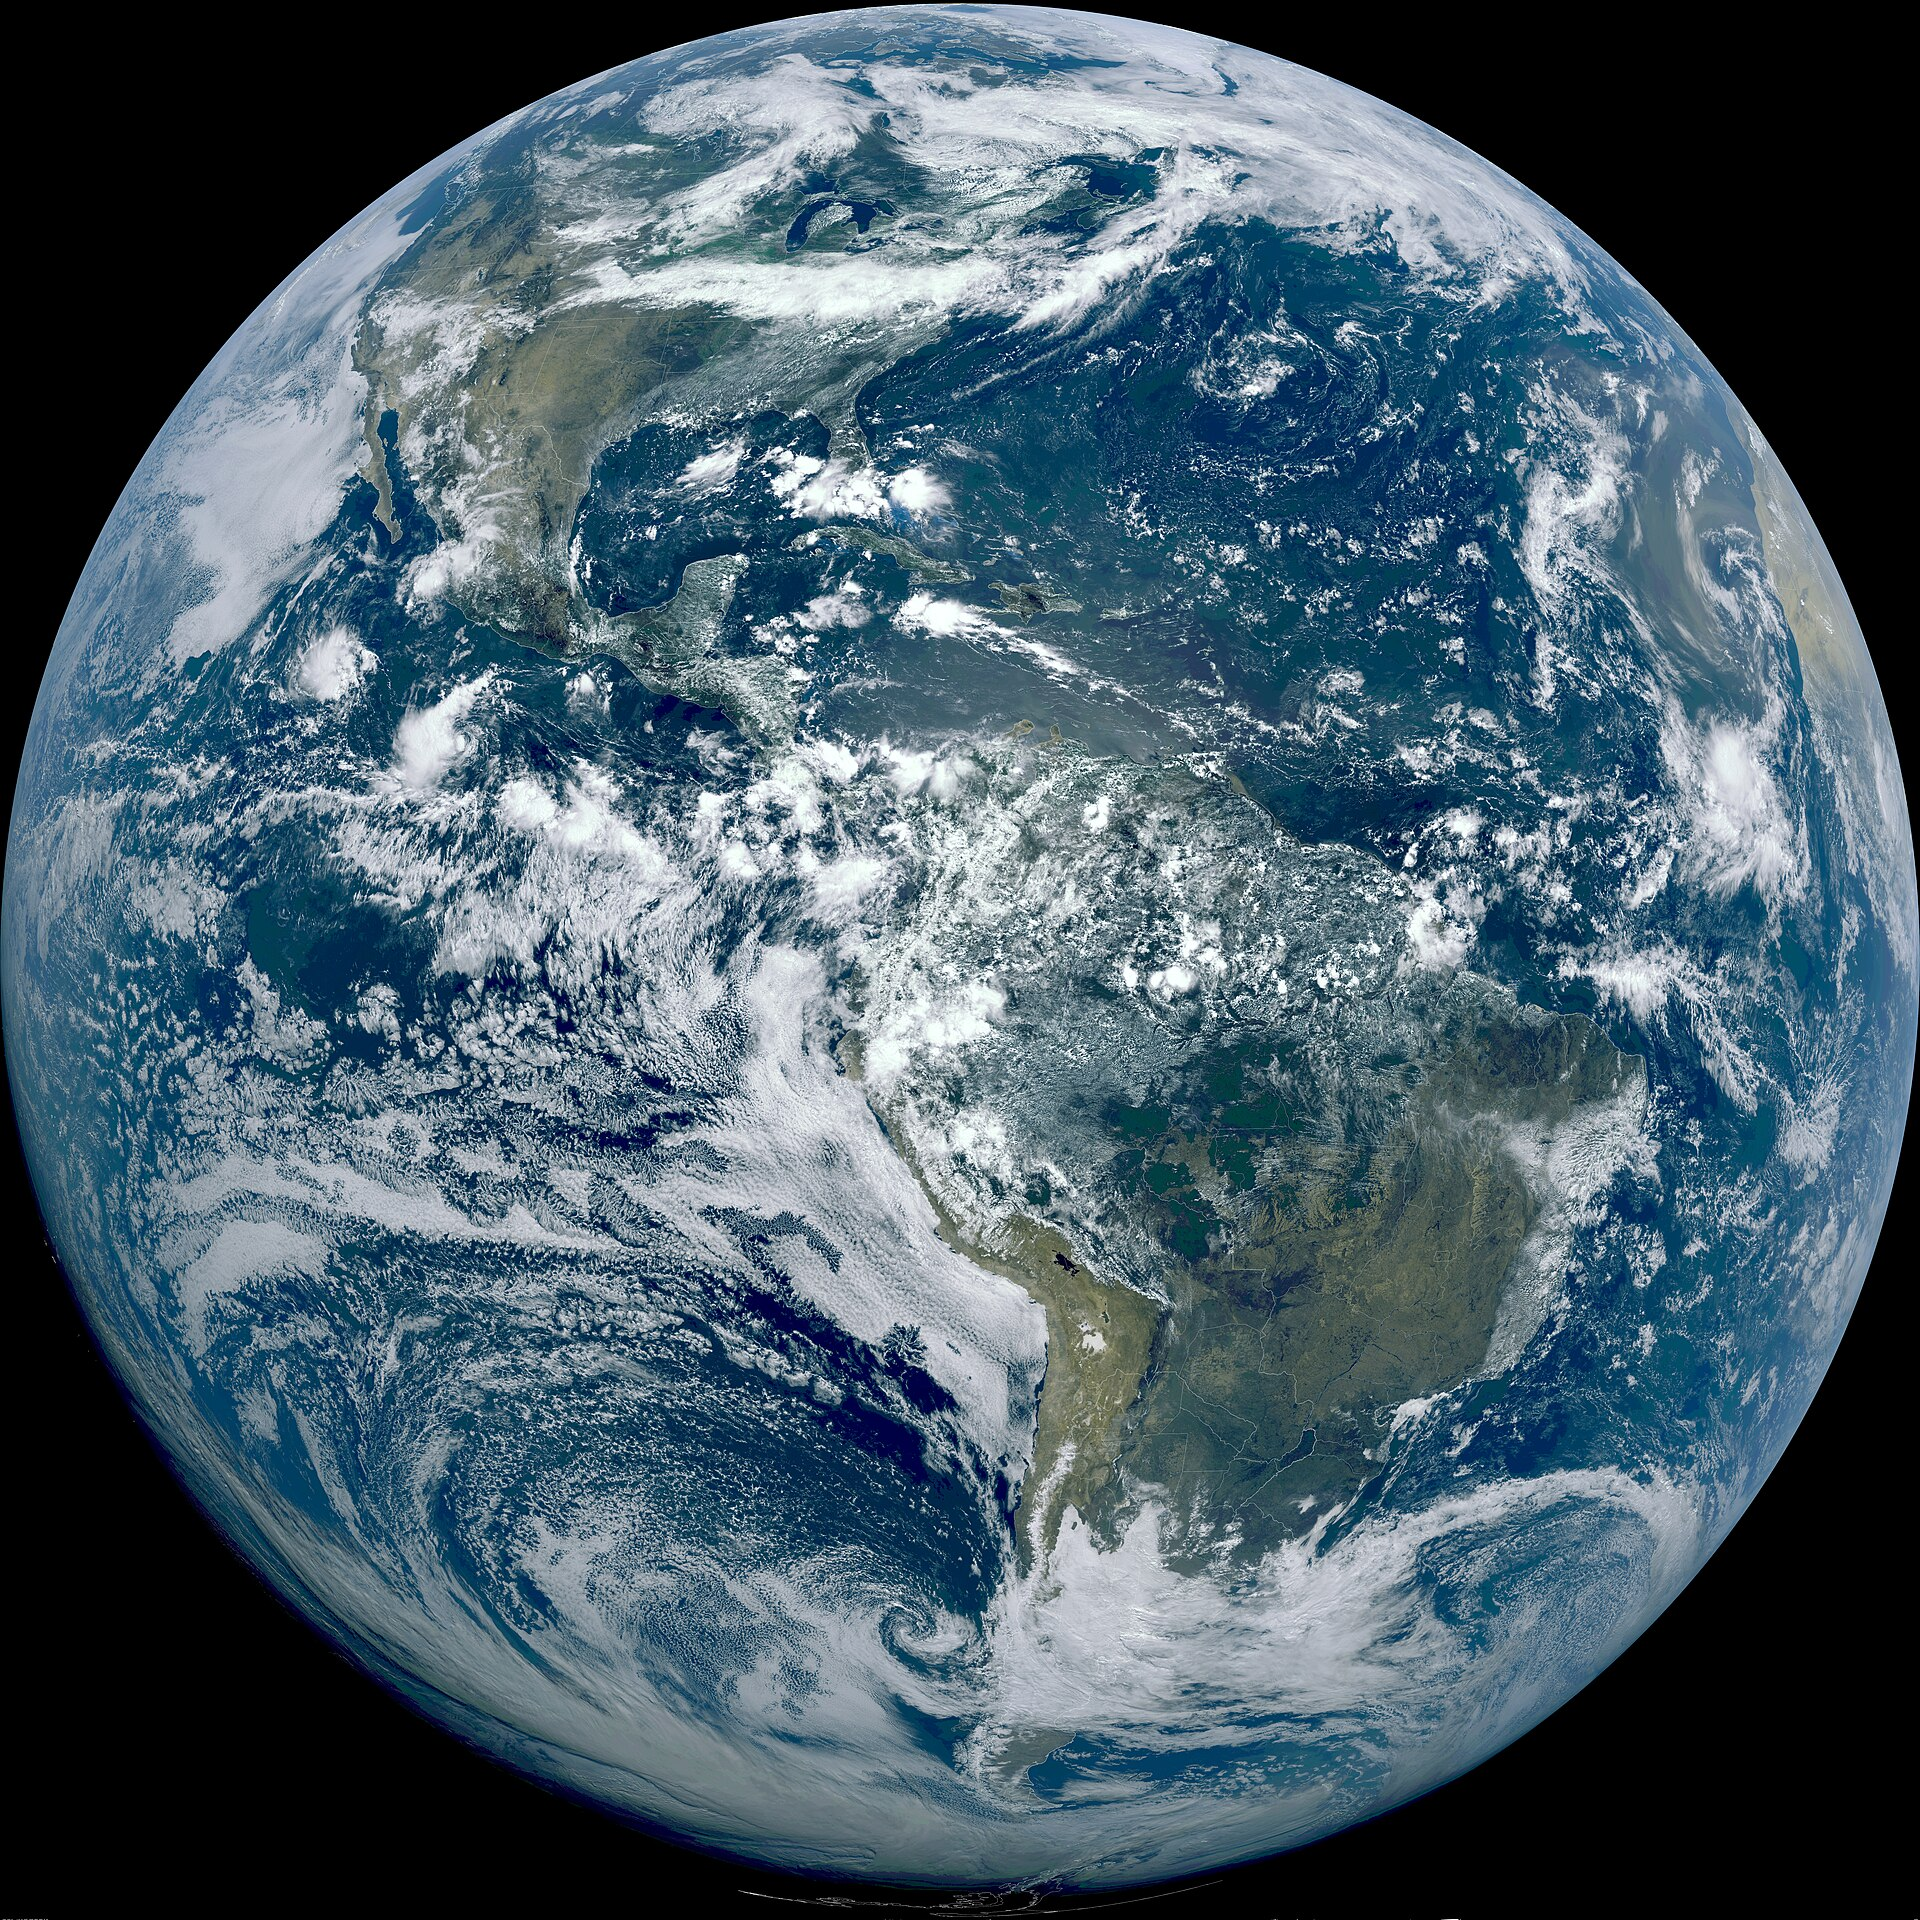
\includegraphics[width=\linewidth]{images/book1/g8-goes-full-disk.jpg}
\end{minipage}\hfill
\begin{minipage}[c]{0.54\linewidth}\raggedright
{\small The Americas seen by the GOES-16 \omterm{def:g1:watching-the-weather:weather}{weather} satellite, high above
the \omterm{def:g3:continents-and-oceans:equator}{equator}, on 26~July 2022. Many \omterm{def:g4:clouds-rain-snow:cloud}{clouds} have formed over
the \omterm{def:g5:weather-and-climate:tropics}{tropics} and the Amazon \omterm{def:g5:weather-and-climate:rainforest}{rainforest}, where warm, damp air rises; far
to the south, in the southern winter, the \omterm{def:g5:natural-hazards:storm}{storms} of the \omterm{def:g8:winds-global-circulation:global-winds}{westerlies} swirl
over the \omterm{def:g2:water-on-earth:ocean}{ocean}. NOAA (public domain, via Wikimedia Commons).}
\end{minipage}
% ledger: commons:goes16, nos:doldrums
\label{fig:g8:winds-global-circulation:goes}
\end{omfigure}

\begin{example}[Four towns, four belts]\label{ex:g8:winds-global-circulation:four-towns}
The four towns of the \omterm{def:g5:weather-and-climate:climate-chart}{climate charts} of \cref{ch:g5:weather-and-climate}
all lie in the \omterm{def:g3:continents-and-oceans:equator}{northern hemisphere}, at very different \omterm{def:g6:latitude-longitude:latitude}{latitudes}. Their
yearly \omterm{def:g4:clouds-rain-snow:precipitation}{rain} and \omterm{def:g4:clouds-rain-snow:precipitation}{snow} follow the belts of the \omterm{def:g8:winds-global-circulation:circulation}{global circulation} (chart
below). Hilo, at \ang{20}\,N, is on an island in the trade-wind belt, in
the middle of the \omterm{def:g2:water-on-earth:ocean}{ocean}, where the \omterm{def:g8:winds-global-circulation:global-winds}{trade winds} pick up water vapour: about
\qty{3000}{mm} fall there in a year. Phoenix, at \ang{33}\,N, lies close to
\ang{30}, under the sinking air: less than \qty{200}{mm}. Seattle, at
\ang{47}\,N, is in the \omterm{def:g8:winds-global-circulation:global-winds}{westerlies}, whose \omterm{def:g5:natural-hazards:storm}{storms} bring about
\qty{1000}{mm} a year, most of it from autumn to spring. Utqia\.gvik, at
\ang{71}\,N, lies under the cold air that sinks near the \omterm{def:g3:continents-and-oceans:poles}{pole}: less than
\qty{150}{mm}, a cold \omterm{def:g5:weather-and-climate:desert}{desert}.
% ledger: data:b1-noaa-normals (totals from figdata/grade-5/climate_charts.py, re-read in figdata/grade-8/rain_by_belt.py), mo:three-cells, nos:doldrums
\end{example}

\begin{omfigure}
\begin{tikzpicture}
\begin{axis}[xbar, width=0.82\linewidth, height=6.4cm, bar width=9pt,
  xmin=0, xmax=3600, ymin=0, ymax=90, ytick={0,30,60,90},
  yticklabels={$0^\circ$, $30^\circ$\,N, $60^\circ$\,N, $90^\circ$\,N},
  xlabel={rain and snow in a year (mm)}, ylabel={latitude},
  axis x line=bottom, axis y line=left, axis line style={-},
  tick label style={font=\scriptsize}, label style={font=\small},
  xtick={0,1000,2000,3000}, scaled x ticks=false, clip=false,
  point meta=explicit symbolic, nodes near coords,
  nodes near coords style={font=\scriptsize, anchor=west}]
  \draw[black!35, dashed] (axis cs:0,30) -- (axis cs:3600,30);
  \draw[black!35, dashed] (axis cs:0,60) -- (axis cs:3600,60);
  \node[font=\scriptsize, black!60, anchor=south east] at (axis cs:3600,1) {rising air: rain};
  \node[font=\scriptsize, black!60, anchor=south east] at (axis cs:3600,30) {sinking air: dry};
  \node[font=\scriptsize, black!60, anchor=south east] at (axis cs:3600,60) {rising air: rain};
  \node[font=\scriptsize, black!60, anchor=north east] at (axis cs:3600,90) {sinking air: dry};
  \addplot[fill=blue!35, draw=blue!60!black] table[x=total_mm, y=lat, meta=name] {figdata/out/grade-8-rain_by_belt-stations.dat};
\end{axis}
\end{tikzpicture}

{\small Yearly \omterm{def:g4:clouds-rain-snow:precipitation}{rain} and \omterm{def:g4:clouds-rain-snow:precipitation}{snow} (averages 1991--2020) of the four towns of the
\omterm{def:g5:weather-and-climate:climate-chart}{climate charts}, placed at their \omterm{def:g6:latitude-longitude:latitude}{latitudes}. The wet towns lie where air
rises, near the \omterm{def:g3:continents-and-oceans:equator}{equator} and near \ang{60}; the dry ones where it sinks,
near \ang{30} and near the \omterm{def:g3:continents-and-oceans:poles}{pole}. NOAA \omterm{def:g5:weather-and-climate:climate}{climate} normals.}
% ledger: data:b1-noaa-normals, mo:three-cells (figdata/grade-8/rain_by_belt.py)
\end{omfigure}

Four towns are only four points: \omterm{def:g1:landscapes-around-us:landform}{mountains}, \omterm{def:g1:landscapes-around-us:water}{coasts} and cold or warm \omterm{def:g2:water-on-earth:ocean}{seas}
also change how much \omterm{def:g4:clouds-rain-snow:precipitation}{rain} a place receives. The belts give the broad
pattern of the \omterm{def:g2:drawing-to-map:map}{map} of \omterm{def:g5:weather-and-climate:climate}{climates}, not the \omterm{def:g4:clouds-rain-snow:precipitation}{rain} of every town.

\section{Exercises}

\begin{exercise}[$\star$]\label{exo:g8:winds-global-circulation:1}
Name the global wind that blows most often: (a) at \ang{15} north;
(b) at \ang{45} south; (c) at \ang{75} north; (d) at \ang{20} south.
Give its direction each time.
\end{exercise}

\begin{exercise}[$\star$]\label{exo:g8:winds-global-circulation:2}
Complete each sentence. (a) Warm air \dots\ and cold air \dots. (b) Under
rising air, the pressure at the ground is \dots. (c) At the ground, the
wind blows from \dots\ pressure towards \dots\ pressure. (d) In the
\omterm{def:g3:continents-and-oceans:equator}{northern hemisphere}, the Earth's rotation turns moving air to the \dots.
\end{exercise}

\begin{exercise}[$\star$]\label{exo:g8:winds-global-circulation:3}
True or false? Correct the false sentences. (a) A \omterm{def:g8:winds-global-circulation:breezes}{sea breeze} blows from
the land to the \omterm{def:g2:water-on-earth:ocean}{sea}. (b) The land warms up faster than the \omterm{def:g2:water-on-earth:ocean}{sea} by day.
(c) The \omterm{def:g8:winds-global-circulation:global-winds}{trade winds} blow from the west. (d) Many great \omterm{def:g5:weather-and-climate:desert}{deserts} lie near
\ang{30} of \omterm{def:g6:latitude-longitude:latitude}{latitude}.
\end{exercise}

\begin{exercise}[$\star$]\label{exo:g8:winds-global-circulation:4}
Draw a \omterm{def:g1:landscapes-around-us:water}{coast} with the \omterm{def:g2:water-on-earth:ocean}{sea} on the left and the land on the right. Add
the Sun, then draw with arrows the loop of air of the \omterm{def:g8:winds-global-circulation:breezes}{sea breeze}. Mark
H and L where the pressure at the ground is high and low.
\end{exercise}

\begin{exercise}[$\star\star$]\label{exo:g8:winds-global-circulation:5}
Use the table of beams in this chapter. (a) At \ang{45}, how much more
ground does a beam cover than at the \omterm{def:g3:continents-and-oceans:equator}{equator}? (b) What percentage of the
\omterm{def:g3:continents-and-oceans:equator}{equator}'s energy does each square metre receive at \ang{60}? (c) At
\ang{75}? (d) Explain in one sentence why the \omterm{def:g3:continents-and-oceans:poles}{poles} are cold.
\end{exercise}

\begin{exercise}[$\star\star$]\label{exo:g8:winds-global-circulation:6}
A boat sails due south through the \omterm{def:g3:continents-and-oceans:equator}{northern hemisphere} and then the
\omterm{def:g3:continents-and-oceans:equator}{southern hemisphere}. (a) Which winds does it meet, in order, from
\ang{70} N to \ang{70} S? (b) Where is it likely to find calm air and
frequent showers? (c) Where are winds light and \omterm{def:g4:clouds-rain-snow:precipitation}{rain} rare?
\end{exercise}

\begin{exercise}[$\star\star$]\label{exo:g8:winds-global-circulation:7}
At a beach, it is \qty{31}{\degreeCelsius} on the \omterm{def:g3:stones-pebbles-sand:sand}{sand} at 3~p.m. and
\qty{22}{\degreeCelsius} over the \omterm{def:g2:water-on-earth:ocean}{sea}. At 3~a.m. it is
\qty{17}{\degreeCelsius} on the land and \qty{21}{\degreeCelsius} over
the \omterm{def:g2:water-on-earth:ocean}{sea}. (a) Which is warmer at 3~p.m.? Which way does the wind blow?
(b) And at 3~a.m.? (c) By how many degrees does the land temperature
change between the two times? And the \omterm{def:g2:water-on-earth:ocean}{sea} temperature? (d) Explain the
difference.
\end{exercise}

\begin{exercise}[$\star\star$]\label{exo:g8:winds-global-circulation:8}
Air flows from the high-pressure belt near \ang{30} N towards the
\omterm{def:g3:continents-and-oceans:equator}{equator}. (a) Without the Earth's rotation, from which direction would
it blow? (b) Which way does the rotation turn it in this \omterm{def:g3:continents-and-oceans:equator}{hemisphere}?
(c) From which direction does it blow then? (d) Answer the same three
questions for the air flowing towards the \omterm{def:g3:continents-and-oceans:equator}{equator} from \ang{30} S.
\end{exercise}

\begin{exercise}[$\star\star$]\label{exo:g8:winds-global-circulation:9}
Explain, step by step, why it \omterm{def:g4:clouds-rain-snow:precipitation}{rains} so often near the \omterm{def:g3:continents-and-oceans:equator}{equator}:
use the words \emph{heated}, \emph{rises}, \emph{cools}, \emph{\omterm{def:g4:clouds-rain-snow:cloud}{clouds}}.
Then explain why there is a \omterm{def:g5:weather-and-climate:desert}{desert} near \ang{25} N in North Africa: use
the words \emph{sinks}, \emph{high pressure}, \emph{dry}.
\end{exercise}

\begin{exercise}[$\star\star$]\label{exo:g8:winds-global-circulation:10}
A sailing ship leaves a port at \ang{40} N on the west \omterm{def:g1:landscapes-around-us:water}{coast} of Europe
for the Caribbean, at \ang{15} N. (a) Which wind would it meet at
\ang{40} N? Would it help the ship sail west? (b) Why should the ship
first sail south? (c) Which wind carries them west, and between
which \omterm{def:g6:latitude-longitude:latitude}{latitudes}? (d) For the return voyage to Europe, which wind should
the ship look for, and at what \omterm{def:g6:latitude-longitude:latitude}{latitude}?
\end{exercise}

\begin{exercise}[$\star\star\star$]\label{exo:g8:winds-global-circulation:11}
At \omterm{def:g6:latitude-longitude:latitude}{latitude} $L$, a beam of sunlight at noon on an equinox covers $1 \div
\cos L$ times the ground it covers at the \omterm{def:g3:continents-and-oceans:equator}{equator} (on a calculator,
$\cos 60^\circ = 0.5$). (a) Check the value for \ang{60}. (b) Using
$\cos 30^\circ \approx 0.866$, check the value for \ang{30}, rounded to
two decimals. (c) Suppose a solar panel lying flat receives
\qty{1000}{W} on each square metre at noon at the \omterm{def:g3:continents-and-oceans:equator}{equator} on that day.
About how much would the same panel receive at \ang{30}? At \ang{60}?
\end{exercise}

\begin{exercise}[$\star\star\star$]\label{exo:g8:winds-global-circulation:12}
In each \omterm{def:g3:continents-and-oceans:equator}{hemisphere}, the \omterm{def:g8:winds-global-circulation:circulation}{global circulation} has three cells. (a) Draw a
side view of the \omterm{def:g3:continents-and-oceans:equator}{northern hemisphere}, with the \omterm{def:g3:continents-and-oceans:equator}{equator} at the bottom and
the \omterm{def:g3:continents-and-oceans:poles}{pole} at the top, and the three cells as loops; show where the air
rises and where it sinks. (b) Mark the high and low pressure belts at
the ground. (c) Add the surface winds of each cell, turned to the right.
(d) Use your drawing to explain why the \omterm{def:g8:winds-global-circulation:global-winds}{westerlies} blow towards the
north-east.
\end{exercise}

\section{Problem: Sailing with the trade winds}

\begin{problem}[{Weekend problem --- a sailing ship crosses the Atlantic
from Cape Verde to Barbados with the north-east trade wind; the route is
measured on the map, the wind is read, and the length of the crossing is
worked out}]
\label{pb:g8:winds-global-circulation:1}
% ledger: data:b1-ne-places, earth:Rmean, nos:trade-winds (figdata/grade-8/trade_route.py; the speed is exercise data)
A sailing ship leaves Praia, in the Cape Verde Islands, for Bridgetown,
in Barbados. The \omterm{def:g2:drawing-to-map:map}{map} shows the route and the trade wind.

\begin{center}
\begin{tikzpicture}
\begin{axis}[ommap, width=12cm, xmin=-75, xmax=-5, ymin=0, ymax=35, axis equal image,
  xtick={-70,-60,-50,-40,-30,-20,-10}, ytick={0,10,20,30},
  tick label style={font=\scriptsize},
  xlabel={longitude (negative = west)}, ylabel={latitude (north)},
  label style={font=\small}, clip mode=individual]
  \addplot[fill=omLithAlluv, draw=black!60, line width=0.3pt] table {figdata/out/grade-8-trade_route-land.dat};
  \addplot[quiver={u=\thisrow{dlon}, v=\thisrow{dlat}}, -{Stealth[length=1.6mm]}, omThm!80, line width=0.7pt]
    table[x=lon, y=lat] {figdata/out/grade-8-trade_route-trades.dat};
  \addplot[omDef, line width=1.3pt, dashed] table {figdata/out/grade-8-trade_route-route.dat};
  \addplot[only marks, mark=*, mark size=2pt, black] table[x=lon, y=lat] {figdata/out/grade-8-trade_route-ports.dat};
  \node[anchor=north, font=\scriptsize\bfseries, fill=white, inner sep=1pt] at (axis cs:-59.6,12.2) {Bridgetown};
  \node[anchor=south, font=\scriptsize\bfseries, fill=white, inner sep=1pt] at (axis cs:-23.5,15.8) {Praia};
\end{axis}
\end{tikzpicture}
\end{center}

\noindent\textbf{Part I --- The route.}\par\nopagebreak
\begin{enumerate}[beginpenalty=10000]
  \item Praia lies at \ang{14.9} N, \ang{23.5} W; Bridgetown at
        \ang{13.1} N, \ang{59.6} W. How many degrees of \omterm{def:g6:latitude-longitude:longitude}{longitude}
        separate them?
  \item Both ports lie close to \ang{14} N. Along this \omterm{def:g6:latitude-longitude:latitude}{parallel}, one
        degree of \omterm{def:g6:latitude-longitude:longitude}{longitude} measures about \qty{108}{km}. About how many
        kilometres is the crossing? Round to the nearest hundred.
  \item Measured exactly on the round Earth, the shortest route is
        \qty{3896}{km}. Is the answer of question 2 a good estimate?
  \item Do the ports lie in the belt of the \omterm{def:g8:winds-global-circulation:global-winds}{trade winds}? Explain.
\end{enumerate}

\noindent\textbf{Part II --- The wind.}\par\nopagebreak
\begin{enumerate}[resume, beginpenalty=10000]
  \item From which direction does the trade wind blow here?
  \item The ship sails towards the west. Does the wind push it forwards,
        backwards or sideways? Explain with the \omterm{def:g2:drawing-to-map:map}{map}.
  \item Why does the trade wind blow in the same direction almost every
        day of the crossing?
  \item On the way back to Europe, why should the captain not try to
        sail east along \ang{14} N?
\end{enumerate}

\noindent\textbf{Part III --- The crossing.}\par\nopagebreak
\begin{enumerate}[resume, beginpenalty=10000]
  \item Suppose the ship averages \qty{7}{km} per hour. How many
        kilometres does it cover in a day of 24 hours?
  \item If the wind died down for 3 days on the way, how many
        kilometres of progress would the ship lose?
  \item With a steady trade wind, how many days does the ship need for
        \qty{3896}{km}? Round to one decimal.
  \item To the nearest whole day, how long does the crossing last? Is
        it more or less than a month?
\end{enumerate}
\end{problem}
